\documentclass[12pt,a4paper]{article}

\usepackage[utf8]{inputenc}

\usepackage[width=190mm,height=272mm,centering]{geometry}

% \usepackage{mathptmx}
\usepackage{palatino}

%\usepackage{chancery}
%\usepackage{antiqua}
%\usepackage{aboensis}
\usepackage{gfsartemisia-euler}
\usepackage[T1]{fontenc}

% \usepackage{fontspec}
% \setmainfont{QTChanceryType}

\usepackage{graphicx}
\usepackage[table]{xcolor}
\usepackage{tikz}
%\usetikzlibrary{decorations.text}
\usepackage[hidelinks]{hyperref}

\pagestyle{empty}

%\newcommand{\logo}{\makebox[56mm][c]{\rule{0mm}{66mm}\raisebox{12mm}{\includegraphics[width=48mm]{logo/aldc-4couleurs-3.pdf}}}}

%\pagecolor{yellow!5}

\usepackage{fontspec}
\usepackage{eurosym}

\begin{document}
\sffamily
\bfseries
%\color{yellow!20}
\parindent=0mm

%%%%%%%%%%%%%% FOND ET LOGOS

\unitlength=1mm
\begin{picture}(0,0)
%\put(-22,-150){\includegraphics[width=212mm]{images/lambris-chene-clair.png}}
%\put(-16,-200){\includegraphics[width=212mm]{images/lambris-chene-clair.png}}
\put(-11,-280){\includegraphics[width=212mm]{../images/Fond-bois-tres-clair-small.jpg}}
%\put(15,-274){\includegraphics[width=140mm]{images/groupe.pdf}}
\put(15,-270){\includegraphics[width=170mm]{../images/groupededanseenligne-ombre.png}}
%\put(-3,-274){\href{https://alevisdanse.github.io}{\includegraphics[width=40mm]{images/qr-code.pdf}}}
%\put(-3,-274){\includegraphics[width=100mm]{images/Exposants.png}}
%\put(20,-274){\includegraphics[width=80mm]{images/Vero'sBoutik.png}}
%\put(90,-210){\includegraphics[width=100mm]{images/Charlie-Gon.png}}
\put(146,-30){\href{https://alevisdanse.github.io}{\includegraphics[height=40mm]{../static/images/logo-aldc-contour-noir.pdf}}}
\put(-6,-35){\href{https://country-rn10-13.webself.net/}{\includegraphics[height=50mm]{../images/LOGO RN10 officiel-fi36141364x430.png}}}
\end{picture}


\vspace*{-20mm}

\begin{center}

\fontsize{96pt}{96pt}
\fontspec{QTOKCorral-Ext}
\selectfont

At Lévis' \\
Saloon \\

\vspace*{20mm}

\fontsize{64pt}{64pt}
\fontspec{QTOKCorral-Ext}
\selectfont

\begin{tabular}{p{0.6\textwidth}@{\hspace*{16mm}}r}
    \raisebox{0mm}{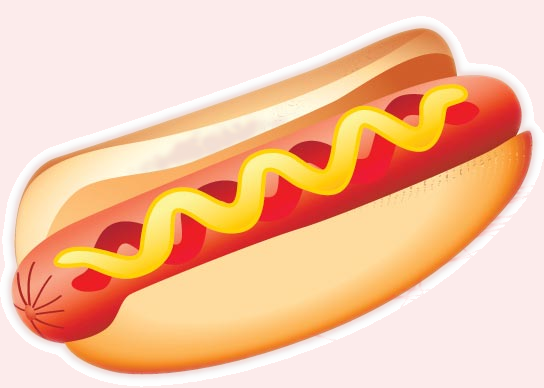
\includegraphics[height=16mm]{../images/hot-dog.png}} Hot Dog  & 3,50 \euro \\

    Pâtisserie \raisebox{0mm}{
\includegraphics[height=16mm]{../images/cake2.png}} & 1 \euro \\

    \raisebox{-2mm}{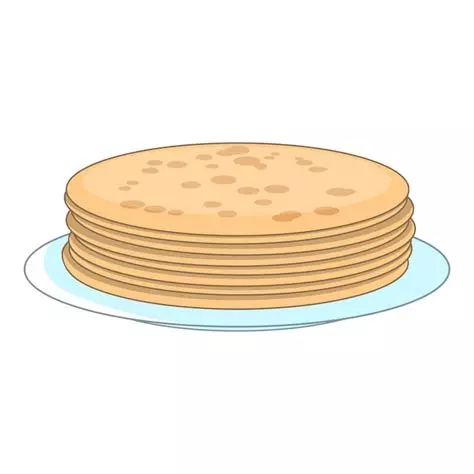
\includegraphics[height=20mm]{../images/crepes.png}} Crêpe Sucre  & 1 \euro \\

    Crêpe Nutella \raisebox{-2mm}{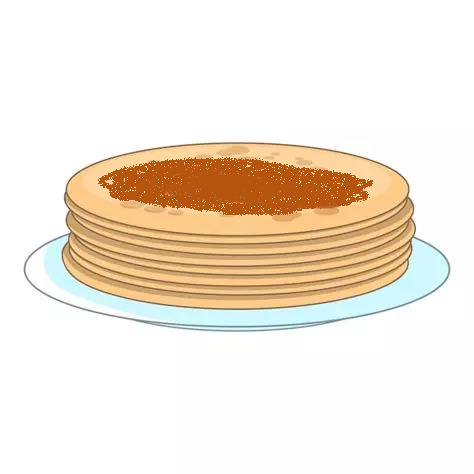
\includegraphics[height=20mm]{../images/crepes-chocolat.png}} & 1,50 \euro \\

    \raisebox{0mm}{
\includegraphics[height=16mm]{../images/beer.png}} Bière & 2,50 \euro \\

    Soda \raisebox{-2mm}{
\includegraphics[height=20mm]{../images/soda2.png}}  & 1,50 \euro \\

    \raisebox{0mm}{
\includegraphics[height=16mm]{../images/water.png}} Eau & 0,50 \euro \\

    Café/Thé \raisebox{0mm}{
\includegraphics[height=16mm]{../images/coffee.png}} & 0,50 \euro \\

  \end{tabular}
\end{center}

\end{document}


% Local variables:
% mode: latex
% TeX-master: t
% TeX-PDF-mode: t
% TeX-engine: luatex
% mode: flyspell
% ispell-local-dictionary: "francais"
% End:
